%% LyX 2.2.2 created this file.  For more info, see http://www.lyx.org/.
%% Do not edit unless you really know what you are doing.
\documentclass[english]{article}
\usepackage[T1]{fontenc}
\usepackage[latin9]{inputenc}
\usepackage{babel}
\usepackage{lipsum}
\usepackage{array}
\usepackage{graphicx}
\usepackage[unicode=true]
 {hyperref}

\makeatletter

%%%%%%%%%%%%%%%%%%%%%%%%%%%%%% LyX specific LaTeX commands.
%% Because html converters don't know tabularnewline
\providecommand{\tabularnewline}{\\}

\makeatother

\begin{document}


\section{Cicuta}

Cicuta, commonly known as water hemlock, is a small genus of four
species of highly poisonous plants in the family Apiaceae. They are
perennial herbaceous plants which grow up to 2.5 meters (8.2 ft) tall,
having distinctive small green or white flowers arranged in an umbrella
shape (umbel). Plants in this genus may also be referred to as cowbane
or poison parsnip. Cicuta is native to temperate regions of the Northern
Hemisphere, mainly North America and Europe, typically growing in
wet meadows, along streambanks and other wet and marshy areas. These
plants bear a close resemblance to other members in the family Apiaceae
and may be confused with a number of other edible and poisonous plants.
The common name hemlock may also be confused with poison hemlock (Conium
maculatum).

Water hemlock is considered one of North America's most toxic plants,
being highly poisonous to humans.{[}1{]} Three members of the genus
contain a toxin named cicutoxin which causes central nervous system
stimulatory effects including seizures following ingestion. Medical
treatment of poisoning may include the use of activated charcoal to
decrease gastrointestinal absorption of the toxic principle along
with supportive care including anticonvulsant drugs such as a benzodiazepine.
High doses of anticonvulsant medicine are often required to halt seizure
activity and further medical care including intubation and mechanical
ventilation may be required.
\begin{center}
\begin{figure}
\begin{centering}
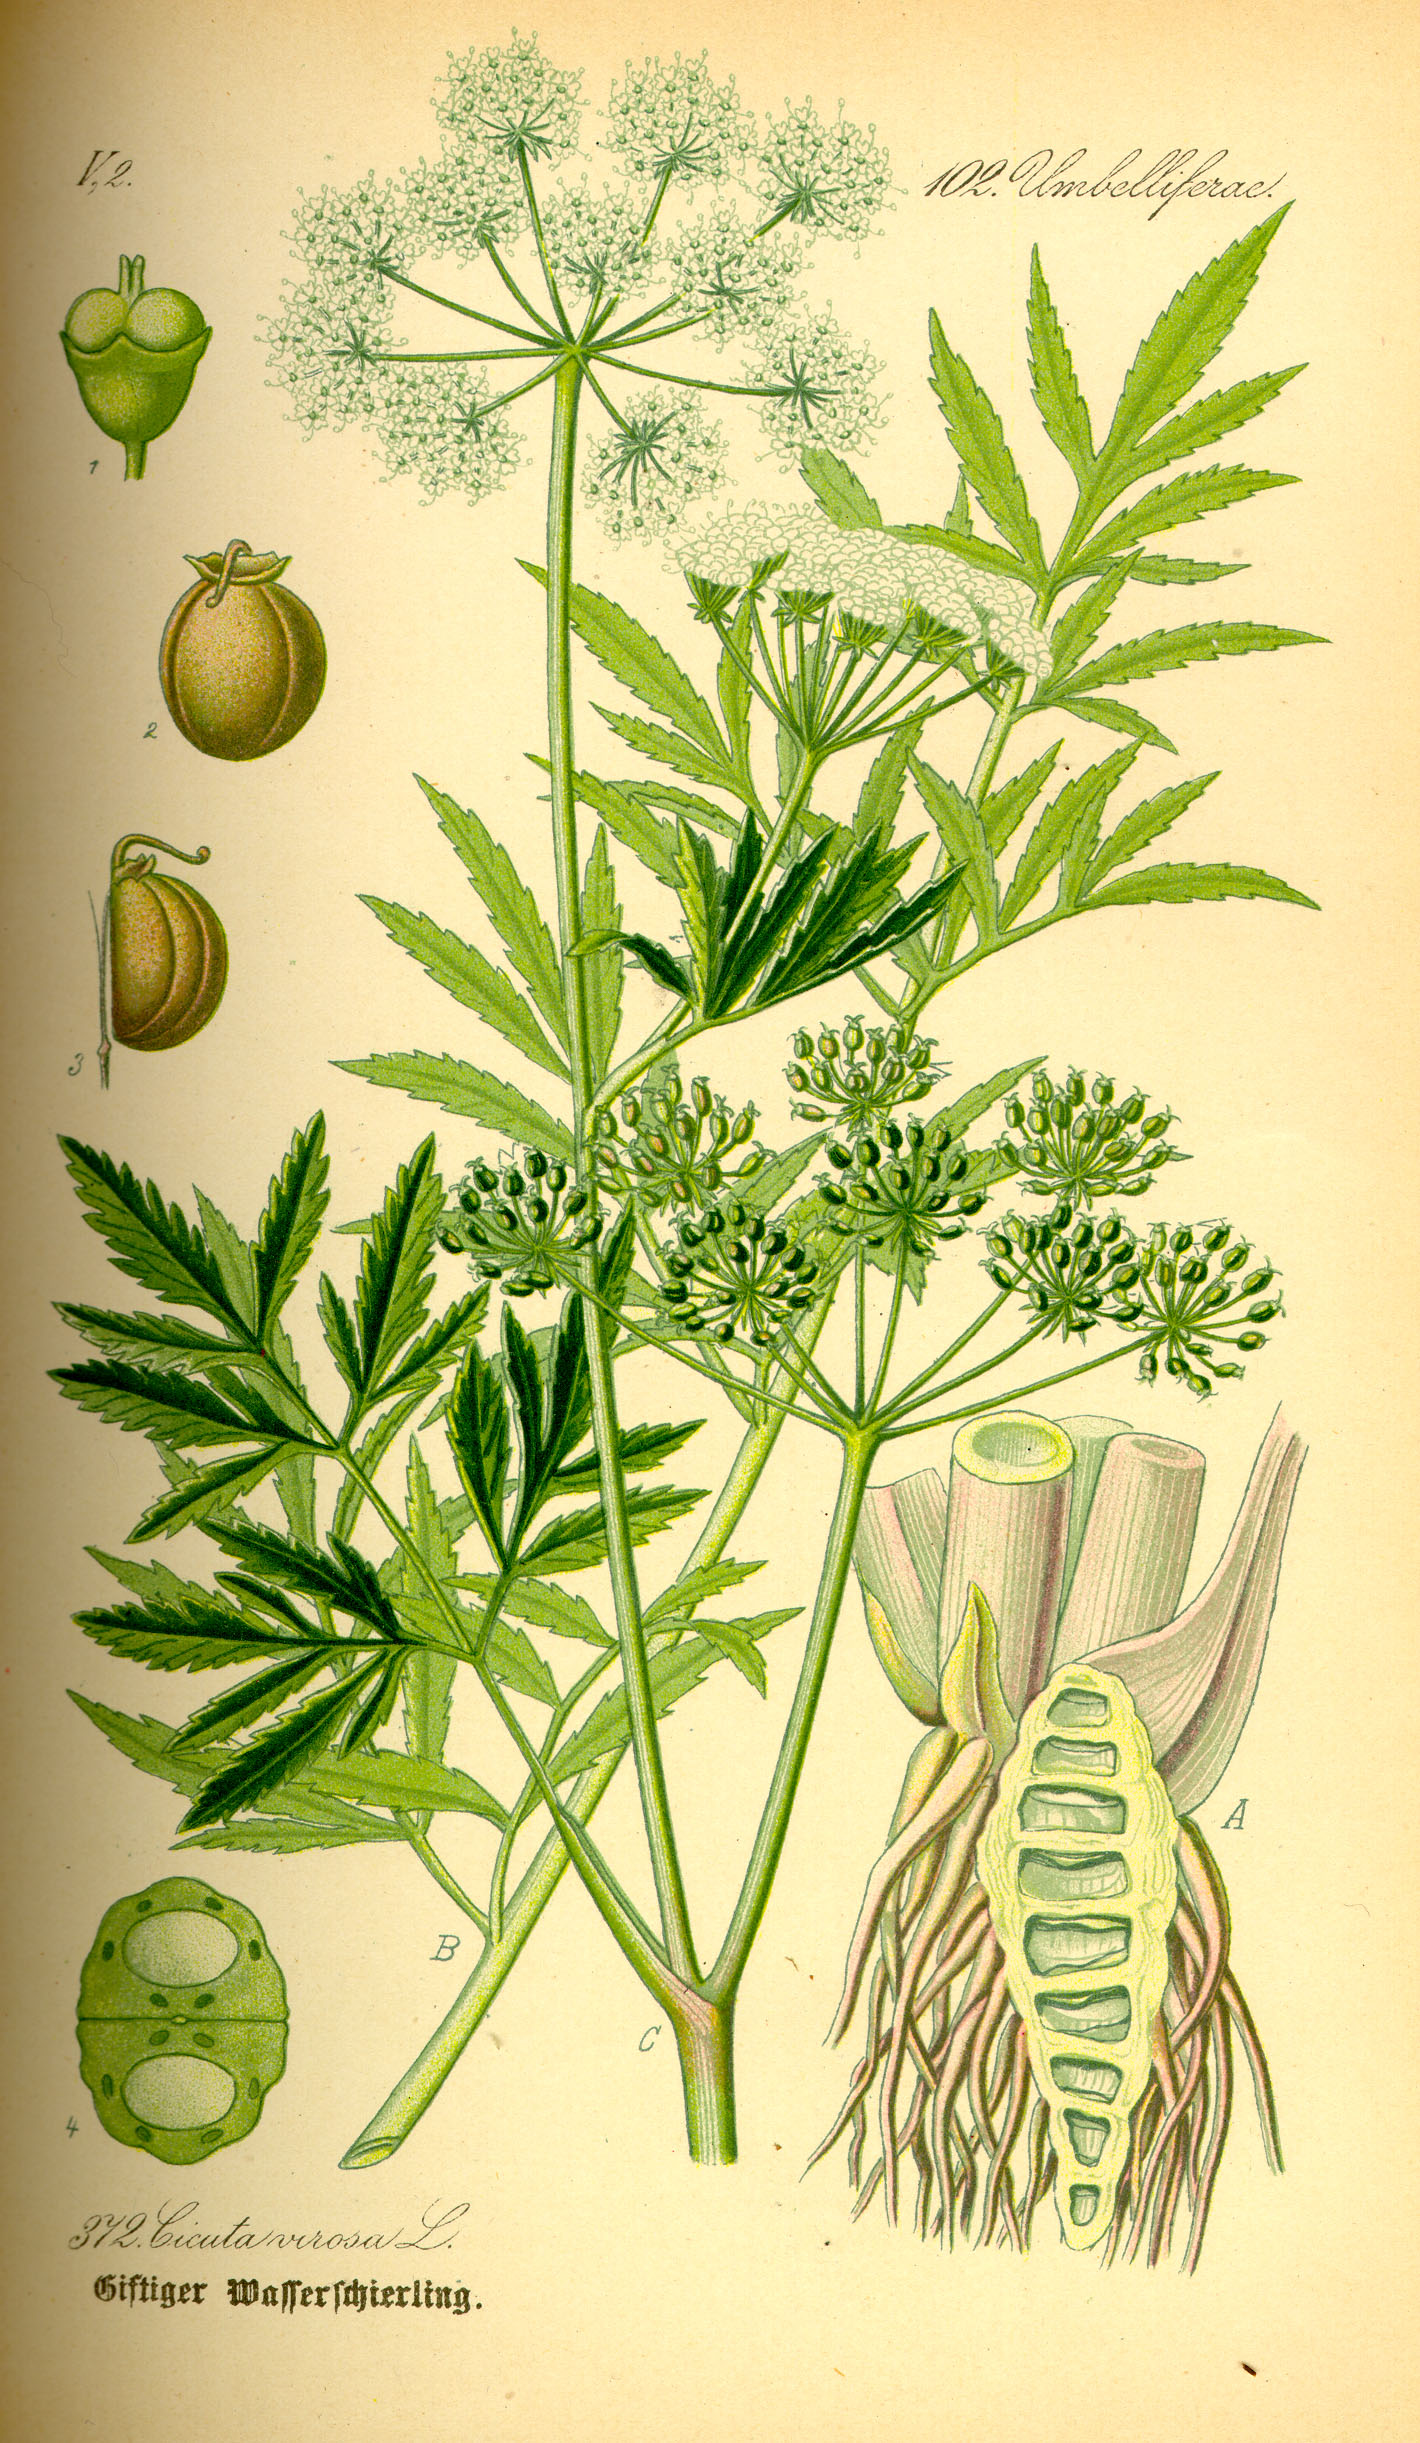
\includegraphics[width=4cm]{IllustrationCicutaVirosa0}
\par\end{centering}
\caption{Cicuta Virosa. Source: \protect\href{https://en.wikipedia.org/wiki/Cicuta}{https://en.wikipedia.org/wiki/Cicuta}}
\end{figure}
\par\end{center}

\subsection{Description}

Cicuta spp. are perennial plants that are all similar in morphology,
growing up to a maximum of 2.5 meters (8.2 ft) in height. The stem
of the plant is branching, erect, smooth and hollow (except for partitions
at the junction of the leaves and stem), sometimes being purple-striped,
or mottled (typically only C. maculata has the purple stripes or spots).
Attached to the base of the stem is a tuberous root with thickened
rootstocks. The rootstocks are multichambered and contain a yellowish
oily liquid which turns reddish brown on exposure to air and emits
a characteristic smell of raw parsnip. The alternate leaves are 2
or 3 pinnately compound and may reach 30 centimeters (12 in) to 90
centimeters (35 in) in length. The leaflets are lanceolate, serrate,
5 centimeters (2.0 in) to 10 centimeters (3.9 in) in length, and sharply
toothed. The plant flowers in spring or early summer; the flowers
are small with green or white petals clustered in an umbrella shape
(umbel) characteristic to this family; the umbel measures 5 centimeters
(2.0 in) to 10 centimeters (3.9 in) across. The plants produce a cylindrical
fruit which is 4 millimeters (0.16 in) to 6 millimeters (0.24 in)
in length.{[}1{]}{[}2{]}{[}3{]} The plant is spread primarily by seeds
which are produced in large numbers and are small in size.{[}2{]}

\subsection{Taxonomy}

The Cicuta genus is one of many genera in the Apiaceae family which
is in the order Apiales. The Apiaceae family is also known as Umbelliferae
and both of these family names are permitted to be used by the International
Code of Botanical Nomenclature.{[}1{]} In Europe, Cicuta was not distinguished
from the similar genus Conium before the year 1500. The first mention
of the genus in the United States was in the eighteenth century.{[}2{]}
Carl Linnaeus formally described three species in 1753.{[}4{]} The
type species is Cicuta virosa.{[}5{]} The genus is now recognized
to comprise four species:{[}6{]}
\begin{center}
\begin{tabular}{|>{\raggedright}p{4cm}|>{\raggedright}p{5cm}|}
\hline 
Species Name & Common Name\tabularnewline
\hline 
\hline 
Cicuta bulbifera L. & bulblet-bearing water hemlock, bulbous water hemlock \tabularnewline
\hline 
Cicuta douglasii (DC.) Coult. \& Rose  & Douglas water hemlock, western water hemlock \tabularnewline
\hline 
Cicuta maculata L.  & spotted cowbane, spotted parsley, spotted water hemlock \tabularnewline
\hline 
Cicuta virosa L. & cowbane, Mackenzie\textquoteright s water hemlock, northern water
hemlock \tabularnewline
\hline 
\end{tabular}
\par\end{center}

Other species names such as Cicuta bolanderi, Cicuta californica,
and Cicuta curtissii are older names now recognized to be varieties
of the widespread, morphologically variable Cicuta maculata.{[}3{]}
Cicuta maculata is now recognized to have four varieties: var. maculata,
var. augustifolia, var. victorinii, and var. bolanderi.{[}6{]} Phylogenetic
analysis using the sequences of nuclear ribosomal DNA internal transcribed
spacer (ITS) loci was not conclusive but seems to show that C. bulbifera
and C. virosa are monophyletic, while C. douglasii may not be. It
was also suggested a specimen from California may warrant recognition
as a distinct species.{[}7{]} Other common names for the genus in
general include poison parsnip, beaver poison, wild carrot, wild parsnip,
and false parsley.{[}8{]}
\end{document}
